\begin{figure}[htbp]
\centering
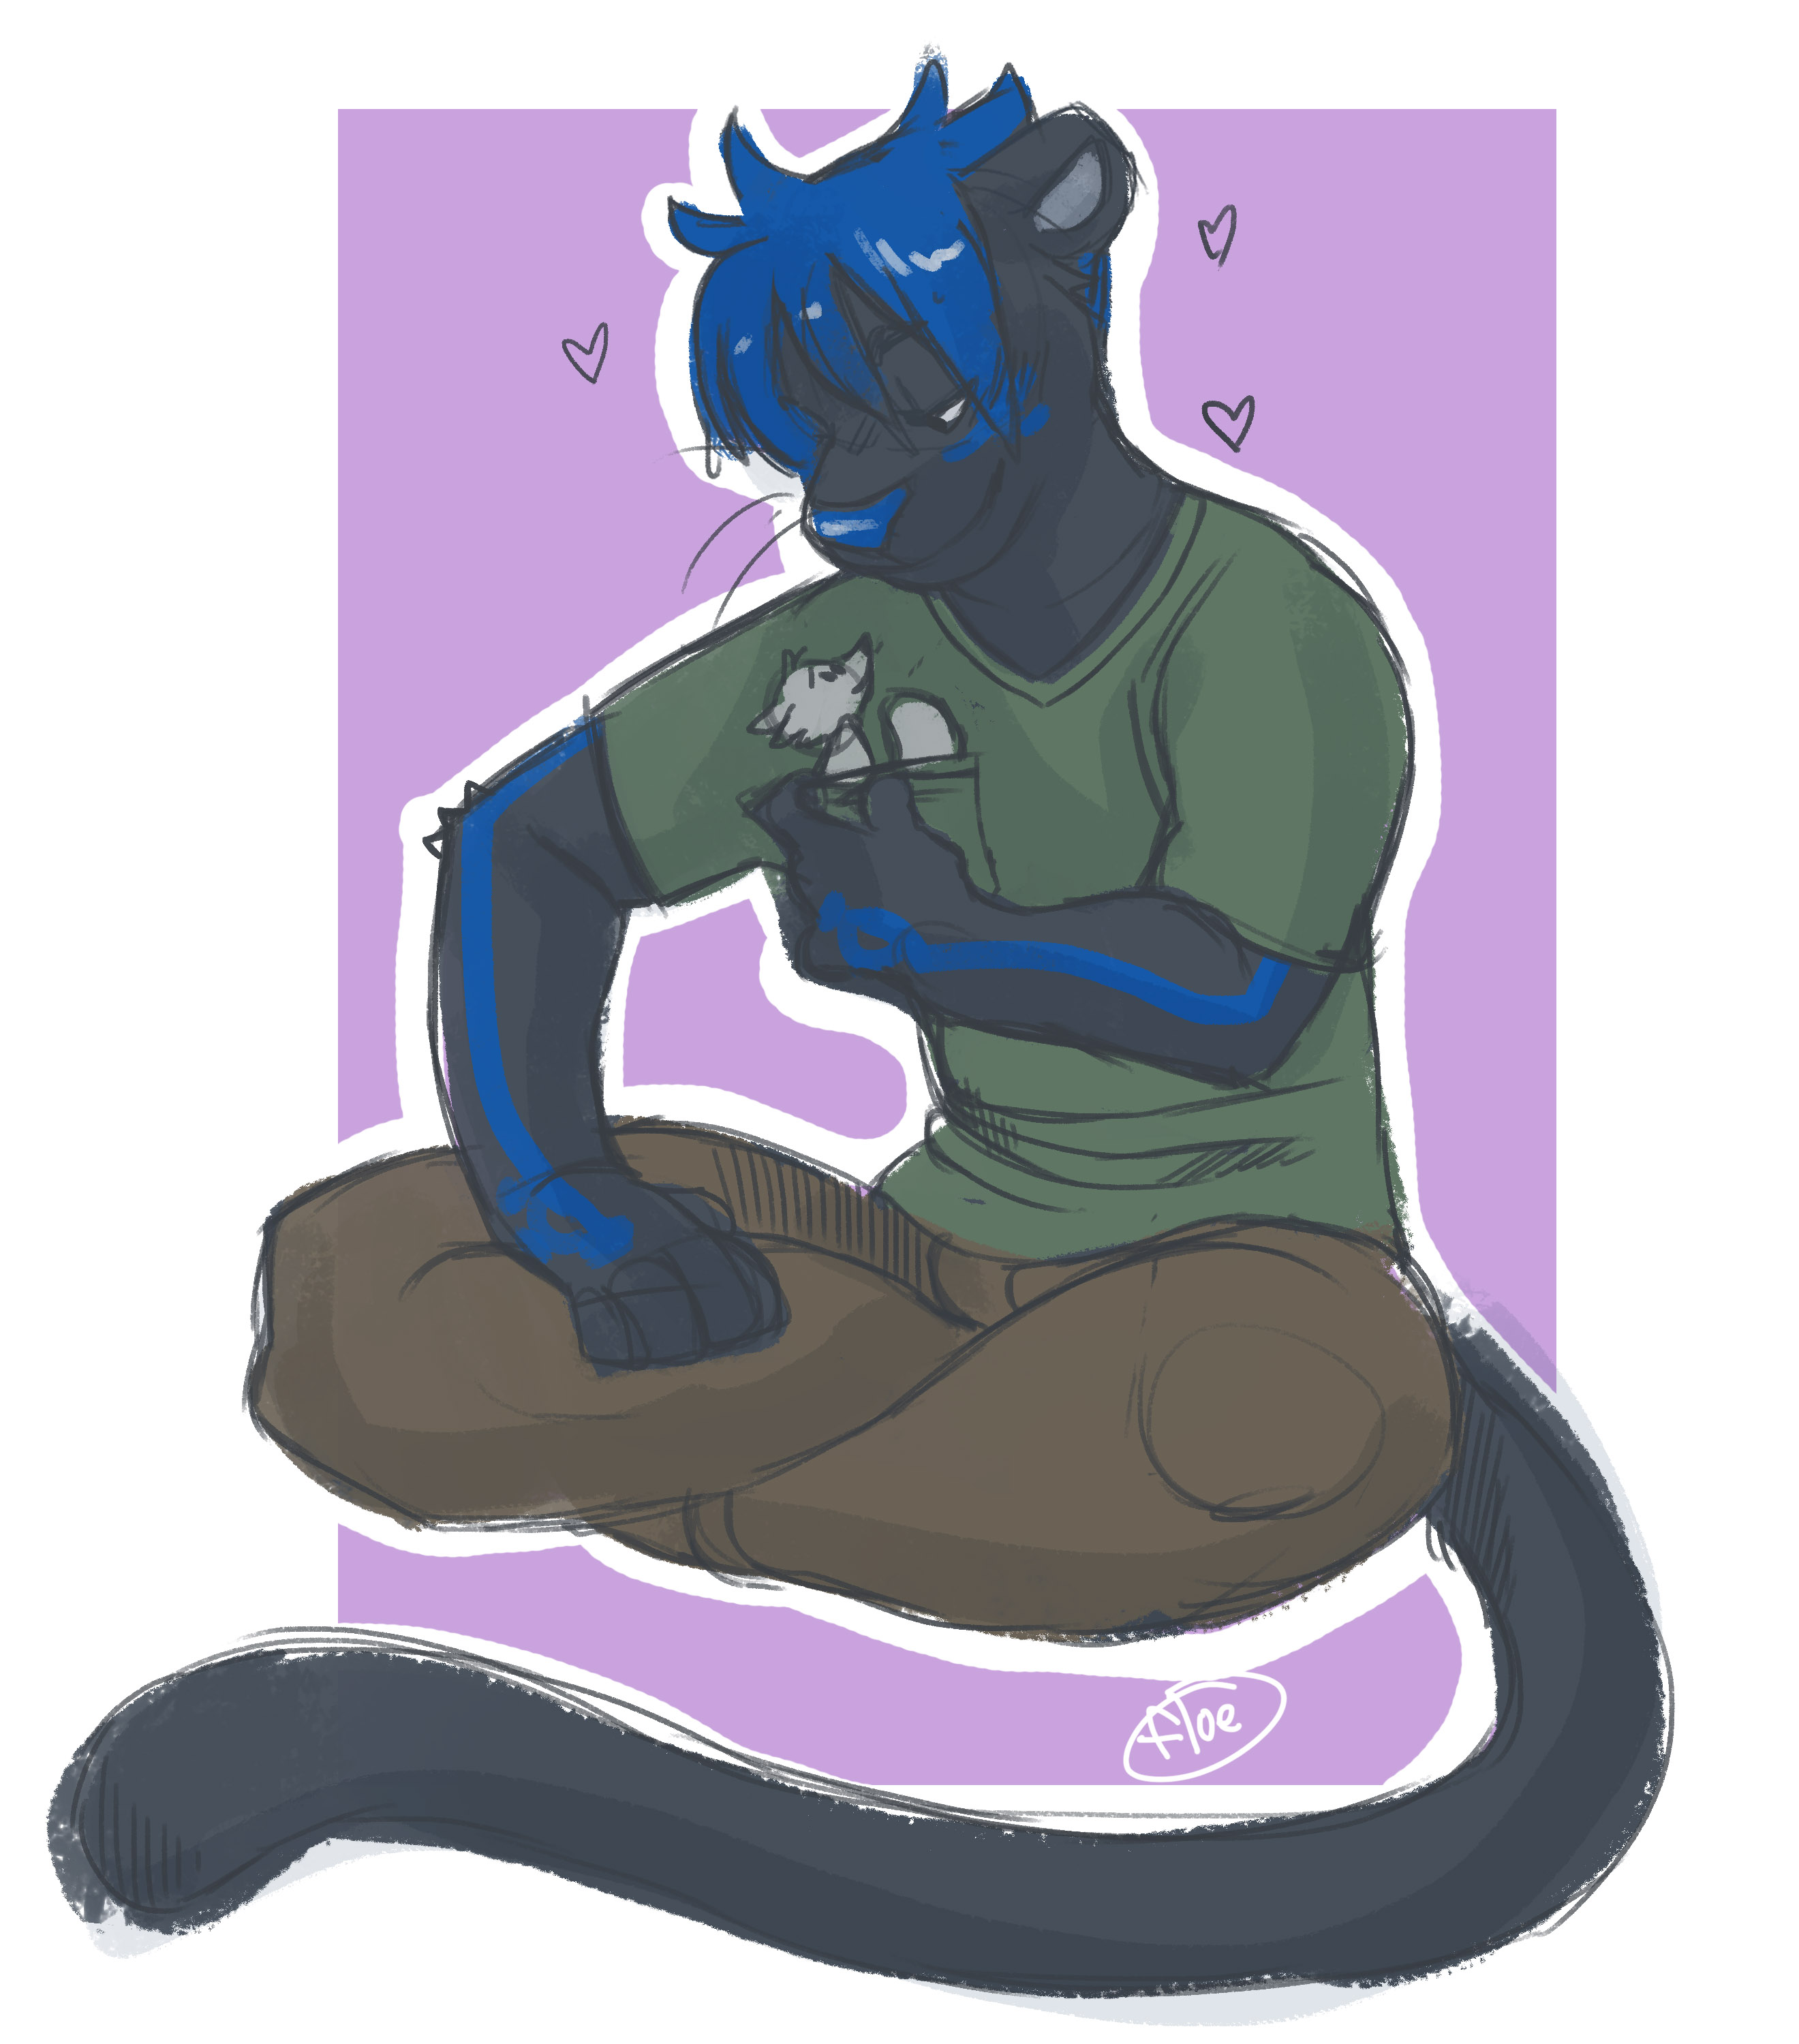
\includegraphics{/assets/furry/trends-within-trends/kb-tinyfoxcomfort1.jpg}
\caption{Tiny foxes: good for comforting}
\end{figure}

It started innocuously enough with a tweet. I don't remember the exact
phrasing of it, but I had been having a rough day and was feeling the
need for some sort of protective affection that I just couldn't quite
find offline; I'm rather tall and so it's hard for me to find a way
that's comfortable for all parties involved to get that sensation of
being held and protected. I think I wound up tweeting something silly to
the effect of ``I just want to curl up in a shirt pocket where it's
warm, cozy, and hidden.'' I suppose I've always been a bit of a sap.

Like most things with far-reaching consequences, this start into the
exploration of the ``micro'' side of the furry fandom had a seemingly
inconsequential beginning. I've mentioned before that, after changing
the ways in which I interacted online, several people treated me as
though I were smaller than I really am (helped, no doubt, by the
combination of text-only interaction and the lack of any specified
height in my character description). With that trivial sentence,
however, it suddenly became explicit, and before long I was interacting
with those around me specifically as a tiny anthropomorphic fox.

\begin{figure}[htbp]
\centering
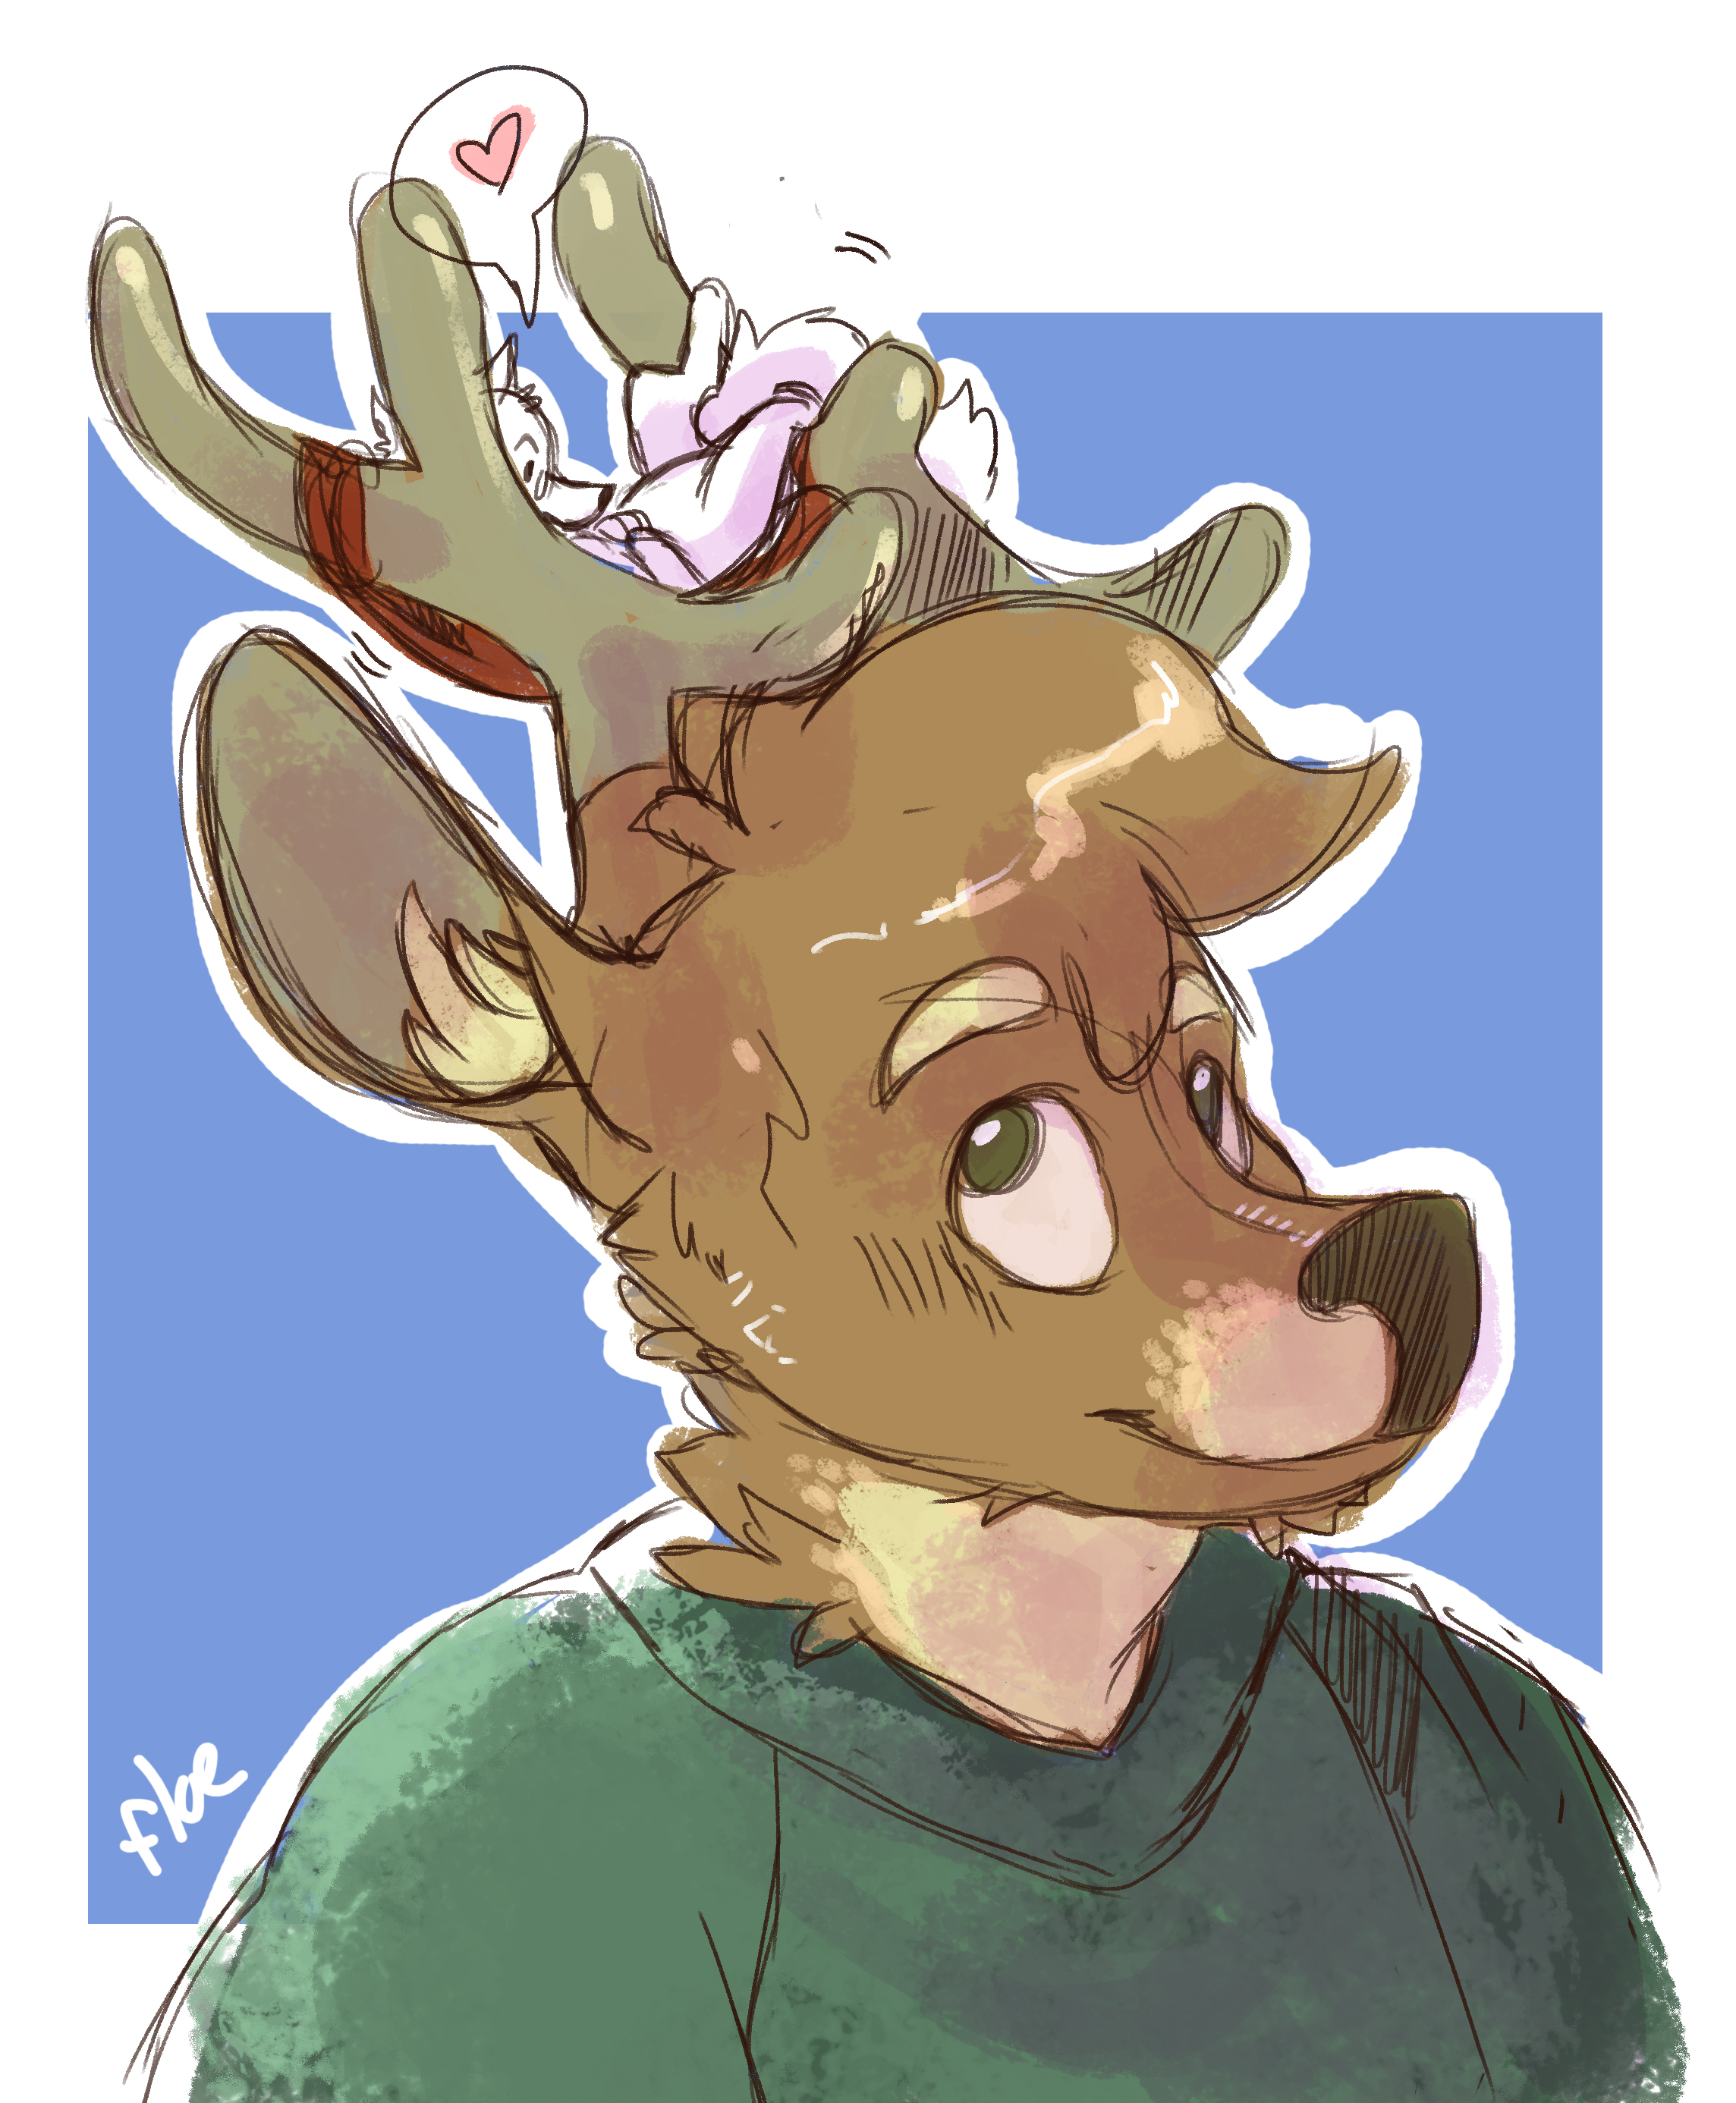
\includegraphics{/assets/furry/trends-within-trends/kb-makyohammock1.jpg}
\caption{Tiny foxes: good for making hammocks in your antlers}
\end{figure}

This is one of those things that feels incredibly silly to write about
in such plain terms. For me, however, it was a new twist on the ways in
which I interacted in familiar surroundings. Everyday objects and
friends became towering structures to scale, and media such as MUCKs and
Twitter became my playground. In short, it felt like a new means of
interacting with the furry community as a whole, akin to the way I felt
when I first discovered the subculture.

And yet, much was still the same. I was still pretending to be a
foxperson on the Internet. My friends-group remained much the same.
Nothing else had really changed in my life, except suddenly, I was part
of a community within a community: a sub-subculture. It came with a
label: micro.

Furry, as a label, is really much too broad to be meaningful except in
the most general of scenarios. It's like saying ``Americans'' when we
know that, with a population of almost 320 million people, that there
are bound to be, for instance, people who describe themselves as
``staunch democrats'' or ``devout Christians'', though, of course, even
those labels are far too broad in some cases. ``Staunch democrats'' does
not take into account the actual politics and core beliefs of an
individual any more than ``devout Christian'' takes into account the
denomination of Christianity of the devout.

\begin{figure}[htbp]
\centering
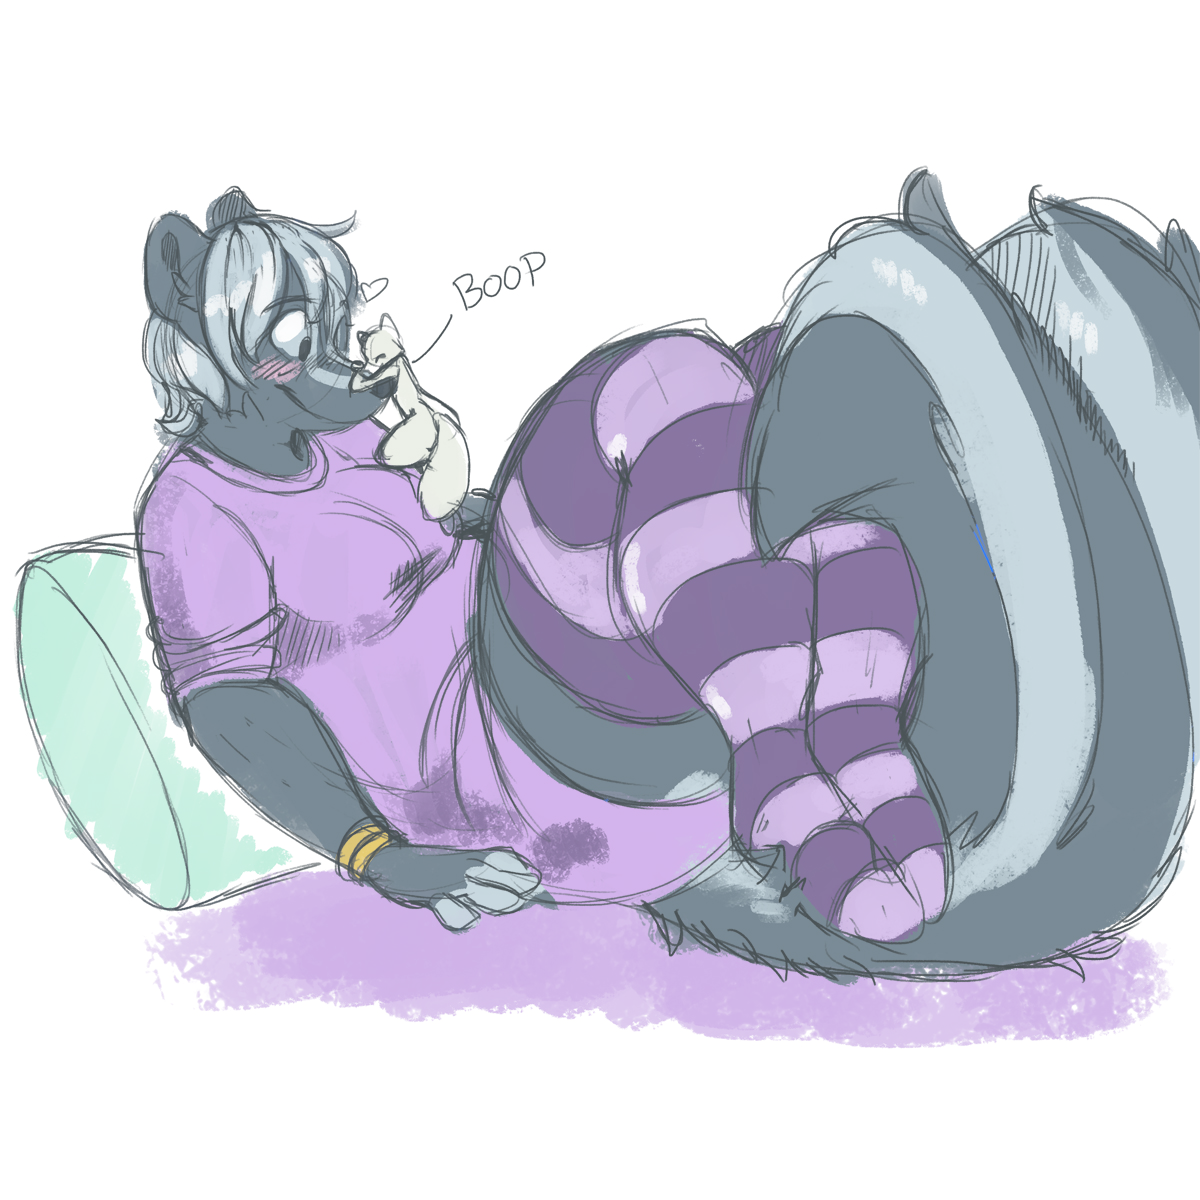
\includegraphics{/assets/furry/trends-within-trends/kb-avery4_7.png}
\caption{Tiny foxes: good for booping noses}
\end{figure}

So it is that we wind up with trends within the larger trend of furry,
and trends within those as well. Micro, as a trend, was a new one to me,
and thus the sensation of newness that reminded me so much of joining
furry in the first place.

I've been a part of various different groups within the larger group of
furry before, of course, just as we all are. I'd identified with gay
furries, then fell out of that as a means of identification as my
sexuality matured. I've identified with trans* and genderqueer furries
as well, as my sense of self has grown over the last several years. The
list goes on, as I'm sure it does for all of us when we boil our
interests down to labels and identities. Why is that, though?

Part of the reason I think that these trends within trends are as big a
thing as they are is that a trend, a label, an identity, or even a kink
can offer one a sense of community. It's all well and good to be a tiny
fox - or genderqueer for that matter - and feel that one has found an
identity that makes one feel comfortable. However, it is the sense of
community, of belonging to a larger group that adds completeness to that
and can help make us feel truly whole.

Also, these interests or identities, when taken up by a group, help to
generate interest and identity in others by the force of their own
presence. That is, while I really rather liked anthropomorphic animals
and playing zoomorphic games while growing up, realizing that there was
a community that bases its very existence off such things led me into
the fandom. Similarly, while I never felt wholly comfortable with my
gender while younger, it was the resources of a community and an
identity that helped me suss out my feelings on the matter.

\begin{figure}[htbp]
\centering
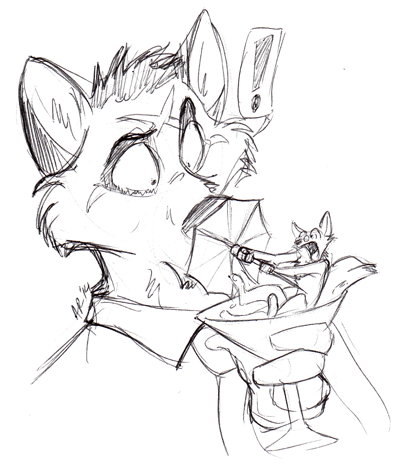
\includegraphics{/assets/furry/trends-within-trends/ao-makyotini-2.png}
\caption{Tiny foxes: not very good for martinis}
\end{figure}

In this way, these trends act as attractors in a system: the closer one
winds up to them, the more likely one is to wind up a part of them. I
think this describes my journey into the furry subculture pretty
accurately: by my presence online, as well as my interests in general, I
wound up close to the community, and my proximity led to my eventual
membership.

Along similar lines, the overlap between these sub-trends within larger
groups such as furry can help introduce one - and thus bring one closer
to - additional groups that one might not find otherwise. For instance,
given my own shared interest in exploring both gender and furry has led
me to the various ways in which the two interact, from the communities
surrounding gender transformation, mixed-gender characters, the gender
gap within the fandom, and so on, all of which I probably would not have
found myself a part of were it not for my previous interests and
identities.

As I alluded to earlier, this is hardly a furry-only phenomenon. After
all, anything from the entirety of the human race down to the individual
level can be divided up into separate trends, likes and dislikes, senses
of identity, and so on. However, as I have mentioned countless times
before, the fact that so much of our interaction takes place online, or
is shifted online after the fact (as would be the case with convention
reports and photos), we leave a vast paper-trail. All one needs to do is
take a peek at someone's profile on any popular art site and see the
groups they consider themselves a member of, the ways in which they
identify (my profile on Weasyl, for instance, has links to my open
source code repositories, which I think speaks to how exciting of a
person I am not).

It's worth taking a moment to step back and investigate the ways in
which you interact with others and identifying the trends that tie you
together. Those ties and the ways in which they interact are what makes
furry so durable a fabric.
